\setchapterpreamble[u]{\margintoc}
\chapter{Viscous Hydrodynamics}
\labch{hydro}

\begin{preview}[]
A schematic review of relativistic hydrodynamics is presented, with emphasis on the {\sffamily DNMR} equations which are implemented in {\sffamily MUSIC}. The Cooper-Fryer formalism and viscous corrections are briefly introduced. A simple parameter search is performed, with shear and w/o bulk viscosity. Best fit to final multiplicities results are shown for a few observables, including elliptic flow.
\end{preview}

\section{Viscous hydrodynamics primer}
\subsubsection*{Ideal hydrodynamics}


\subsubsection*{Dissipative hydrodynamics}


\subsubsection*{Kinetic theory}


\section{Post-hydrodynamics}
\subsubsection*{Cooper-Fryer prescription}
As the {\sffamily QGP} expands, the medium becomes more dilute and its temperature decreases, eventually leading to a phase transition from a state of deconfined quarks and gluons to a hadron gas and then to reconfinement into hadrons.\sidenote{The hadronization begins at the edge of the medium and gradually reaches the central region.}The transition between a hydrodynamic description in terms of the energy-momentum tensor and the subsequent produced particles,\sidenote{Usually referred to as particlization.}is assumed to take place at a given temperature\sidenote{Which is the freeze-out temperature, denoted as $T_\text{fo}$.}for all species. The points at which the particlization temperature is reached form a 4-dimensional hypersurface $\Sigma$. Equipped with a microscopic distribution function,\sidenote{Arising from kinetic theory. Here $i$ is the species index.}one may compute the number of points crossing this hypersurface as\sidenote{Where $g_i$ is the degeneracy of species $i$, $n_i^\mu$ represents the number current, $E_{\vec{p}}$ obeys the relation $E^2_{\vec{p}}=\vec{p}^2+m^2$ and $d^3\Sigma_\mu$ is the surface element oriented along the orthogonal direction from the hypersurface $\Sigma$.}
\begin{align*}
    N_{i}=\int\limits_{\Sigma} d^{3} \Sigma_{\mu}(x)  \underbrace{\frac{g_i}{(2 \pi)^{3}}\int\frac{d^3\vec{p}}{E_{\vec{p}}} p^{\mu} f_{i}(x, p)}_{\mathclap{\textstyle n_i^\mu(x)}}.
\end{align*}
From this one may deduce the {\sffamily\color{ming} Cooper-Fryer} formula\sidenote{This conversion of the hydrodynamic energy-momentum tensor to particles conserves the energy and the number of particles.}\cite{cooperfryer}
\begin{align*}
    \frac{d N_i}{d^{3} \vec{p}}=\frac{g_i}{(2 \pi)^{3}} \int\limits_{\Sigma}   \frac{d^{3}\Sigma_{\mu}p^{\mu}}{E_{\vec{p}}}f_i(x,\vec{p}) ,
\end{align*}
with the distribution function given by\sidenote{The equilibrium distribution function is the Bose-Einstein or Fermi-Dirac distribution
\begin{align*}
    f_\text{eq}(x, \vec{p})=\dfrac{1}{\exp{\dfrac{p \cdot u}{T}} \mp 1}.
\end{align*}
} 
\begin{align*}
    f(x,\vec{p})=f_\text{eq}(x,\vec{p})+\delta f_\text{shear}(x,\vec{p})+\delta f_\text{bulk}(x,\vec{p}).
\end{align*}
The shear correction is chosen to take the quadratic form \cite{dusling} for all hadron species\sidenote{The shear correction must be a scalar constructed with $\pi^{\mu\nu}$.}
\begin{align*}
    \delta f_{\text {shear}}(x, \vec{p})=f_\text{eq}\left(1\pm f_\text{eq}\right) \frac{\pi_{\mu \nu} p^{\mu} p^{\nu}}{2\left(\varepsilon_{0}+P_{0}\right) T^{2}},
\end{align*}
whereas the bulk correction\sidenote{Where the speed of sound is given by
\begin{align*}
    c_{s}^{2} \overset{\Delta}{=}\frac{\partial P_{0}}{\partial \varepsilon_{0}}.
\end{align*}
}, derived using the first-order Chapman-Enskog theory within the relaxation time approximation \cite{paquetbulk, bozek}, is species dependent
\begin{fullwidth}
\begin{align*}
    \delta f_{\text {bulk}}(x, \vec{p})=-f_\text{eq}\left(1\pm f_\text{eq}\right) \frac{C_{\text {bulk}}}{T}\left[\frac{m^{2}}{3(p \cdot u)}-\left(\frac{1}{3}-c_{s}^{2}\right)(p \cdot u)\right] \Pi,
\end{align*}
\end{fullwidth}
with the bulk coefficient expressible as
\begin{fullwidth}
\begin{align*}
    \frac{T}{C_{\text {bulk }}}=\frac{1}{3} \sum_{i} g_{i} m_{i}^{2} \int \frac{d^{3} \vec{k}}{(2 \pi)^{3} E_{\vec{k}}} f_{i, \text{eq}}\left(1 \pm f_{i, \text{eq}}\right)\left[\frac{m_{i}^{2}}{3 E_{\vec{k}}}-\left(\frac{1}{3}-c_{s}^{2}\right) E_{\vec{k}}\right].
\end{align*}
\end{fullwidth}
Afterwards, the number of particles in each cell is sampled according to a Poisson distribution.\sidenote{More details about the sampling procedure and a pedagogical derivation for the dissipative corrections to the distribution function may be found at \cite{ryu}.}The particle spectra resulting from Cooper-Fryer may not directly be compared to experimental data since after particilization, the resulting particles may decay or suffer rescatterings. 

\subsubsection*{General setup}
The events resulting from {\sffamily Curraun}, a {\sffamily Python} based code for computing Glasma fields, are coupled, via energy density and flow velocity obtained from the Landau matching, to {\sffamily MUSIC} \cite{paquetbulk, schenkemusic1, schenkemusic2}, a code\sidenote{Publicly available at \url{https://github.com/MUSIC-fluid/MUSIC} with an user manual at \url{https://webhome.phy.duke.edu/~jp401/music_manual/index.html}}for simulating relativistic heavy-ion collisions, using relativistic second-order viscous hydrodynamics, written in {\sffamily C}\texttt{++}. The most-recent hybrid simulations with {\sffamily CGC} based initial conditions given as input to {\sffamily MUSIC} also include a post-particlization stage\sidenote{In \cite{ryubulk}, it was emphasized that including rescatterings bring significant improvements only for protons and multi-strange particles.}simulated with {\sffamily UrQMD}. Nevertheless, in this work, only the decays of unstable particles shall be considered.\sidenote{{\sffamily MUSIC} is also equipped with resonance decay routines fetched from {\scshape Azhydro} \cite{kolbaz}.} \\
The most important parameters which were provided to {\sffamily MUSIC} as input shall be summarized below. Some parameters have fixed values throughout this study:

\vspace{0.5cm}

\fancybox{ming}{$\tau_\text{switch}$}{
The proper time at which the initial stage is stopped and the hydrodynamic evolution begins. In the current work, it is fixed at $\tau_\text{switch}=0.4$ fm/c.
}
\fancybox{ming}{{\sffamily EoS}}{
The equation of state for the {\sffamily QGP}. We shall employ \texttt{"s95p-v1-PCE"}, constructed by interpolating between {\sffamily HRG} at low temperatures and lattice {\sffamily QCD} {\sffamily EoS} \cite{qcdeos}, with partial chemical equilibrium at $T_\text{chem}=150$ MeV.
}
\fancybox{ming}{$\zeta/s$}{
The specific bulk viscosity. It is hard-coded in {\sffamily MUSIC} and parametrized with respect to temperature \cite{ryuimpbulk, ryubulk}, with a maximum around the {\sffamily QCD} phase transition temperature $T_\text{peak}=180$ MeV.
}
whereas others are allowed to run freely in a certain range:
\fancybox{tealblue}{$s_\text{factor}$}{
The normalization factor for the initial energy density. This parameter is allowed to vary within the range $s_\text{factor}= 0.5\divisionsymbol 2.0$.
}
\fancybox{tealblue}{$\eta/s$}{
The specific shear viscosity. We assume a temperature independent value tuned between $\eta/s=0.08 \divisionsymbol 0.24$ when only shear viscosity corrections are considered and $\eta/s= 0.02 \divisionsymbol 0.1$ when bulk viscosity is also included.
}

% \begin{note}
% \begin{fullwidth}
% \zeta / s(T)=0.9 \times\begin{cases}
% 0.9 \exp{\left(\dfrac{T}{T_{\mathrm{peak}}}-1\right) \Big/ 0.0025}+0.22 \exp{\left(\dfrac{T}{T_{\mathrm{peak}}}-1\right)\Big / 0.022}+0.03 & \text { if } T<0.95 T_{\mathrm{peak}} \\
% -13.77\left(\dfrac{T}{T_{\mathrm{peak}}}\right)^{2}+27.55\left(\dfrac{T}{T_{\mathrm{peak}}}\right)-13.45 & \text { if } 0.95 T_{\mathrm{p}}<T<1.05 T_{\mathrm{peak}} \\
% 0.025 \exp{-\left(\dfrac{T}{T_{\mathrm{peak}}}-1\right) \Big/ 0.025}+0.25 \exp{\left(\dfrac{T}{T_{\mathrm{peak}}}-1\right)\Big / 0.13}+0.001 & \text { if } T>1.05 T_{\mathrm{peak}}
% \end{cases}
% \end{fullwidth}
% \end{note}
\fancybox{tealblue}{$T_\text{fo}$}{
The kinetic freeze-out temperature, at which the Cooper-Fryer formula is applied for conversion to particles, allowed to take values within $T_\text{fo}=100\divisionsymbol 180$ MeV.
}
The strategy for extracting relatively realistic values for the free parameters is the following: firstly, we average all the events from a certain centrality class, as obtained from {\sffamily Curraun}, since performing an event-by-event search for optimal parameters would be time expensive and using averaged initial conditions should provide reasonable results for spectra and final multiplicities; next, the averaged initial distributions\sidenote{More concisely, averaged input files with energy density and flow velocity for $0-5\%$, $5-10\%$, $10-20\%$, $20-30\%$ and $30-40\%$}are provided as input for {\sffamily MUSIC} with sufficiently many values for $s_\text{factor}$, $\eta/s$ and $T_\text{fo}$; afterwards, the set of parameters which best fit\sidenote{Which give the smallest $\chi^2$.}the finally measured multiplicities\sidenote{For pions, kaons and protons.}are chosen; these values are then used to perform event-by-event simulations for all centralities;\sidenote{With $300$ events per centrality class.}lastly, we compare the results from this hybrid approach to experimental data. \\
Among experimentally measured observables such as $p_T$ spectra and particle multiplicities, it is also instructive to study the flow coefficients\sidenote{We shall focus on the elliptic flow $v_2$, which is considered to be an important signature of {\sffamily QGP}.}which arise from such an hybrid approach. From the Fourier expansion\sidenote{Where $\Phi$ is the azimuthal angle and $\Psi_n$ denotes the event-plane angle.}
\begin{align*}
    \frac{dN}{d\Phi}=\frac{N}{2 \pi} \left[1+2 \sum_{n} v_{n} \cos \left[n\left(\Phi-\Psi_{n}\right)\right]\right],
\end{align*}
one may extract flow coefficients as\sidenote{They reflect the final momentum anisotropy, which may be caused by initial spatial anisotropies.}
\begin{align*}
    v_{n}\overset{\Delta}{=}\left\langle\cos \left[n\left(\Phi-\Psi_{n}\right)\right]\right\rangle.
\end{align*}
Event-by-event fluctuations in the initial energy density profile, which may display higher deformations, gives rise to higher order harmonics.\sidenote{As showed in \cite{schenkeflow}, where high order flow coefficients are well described by employing {\sffamily EbE} fluctuating initial conditions.}The study of flow coefficients enables the extraction of fundamental properties of the {\sffamily QGP}, such as transport coefficients or the equation of state. Nevertheless, such a study requires a very good description of every collision stage.

\section{Results}
\subsubsection*{Shear viscosity}
The minimal bayesian study described previously lead to the best fit parameters $s_\text{factor}=1.6$, $\eta/s=0.24$ and $T_\text{fo}=180$ MeV for the case when only the shear dissipative corrections are taken into account. Before looking at the final results, it is perhaps instructive to see\sidenote{By keeping all the other parameters at the best fit values.}how varying the shear viscosity of freeze-out temperature affects the spectra. 

\begin{figure}[!hbt]
	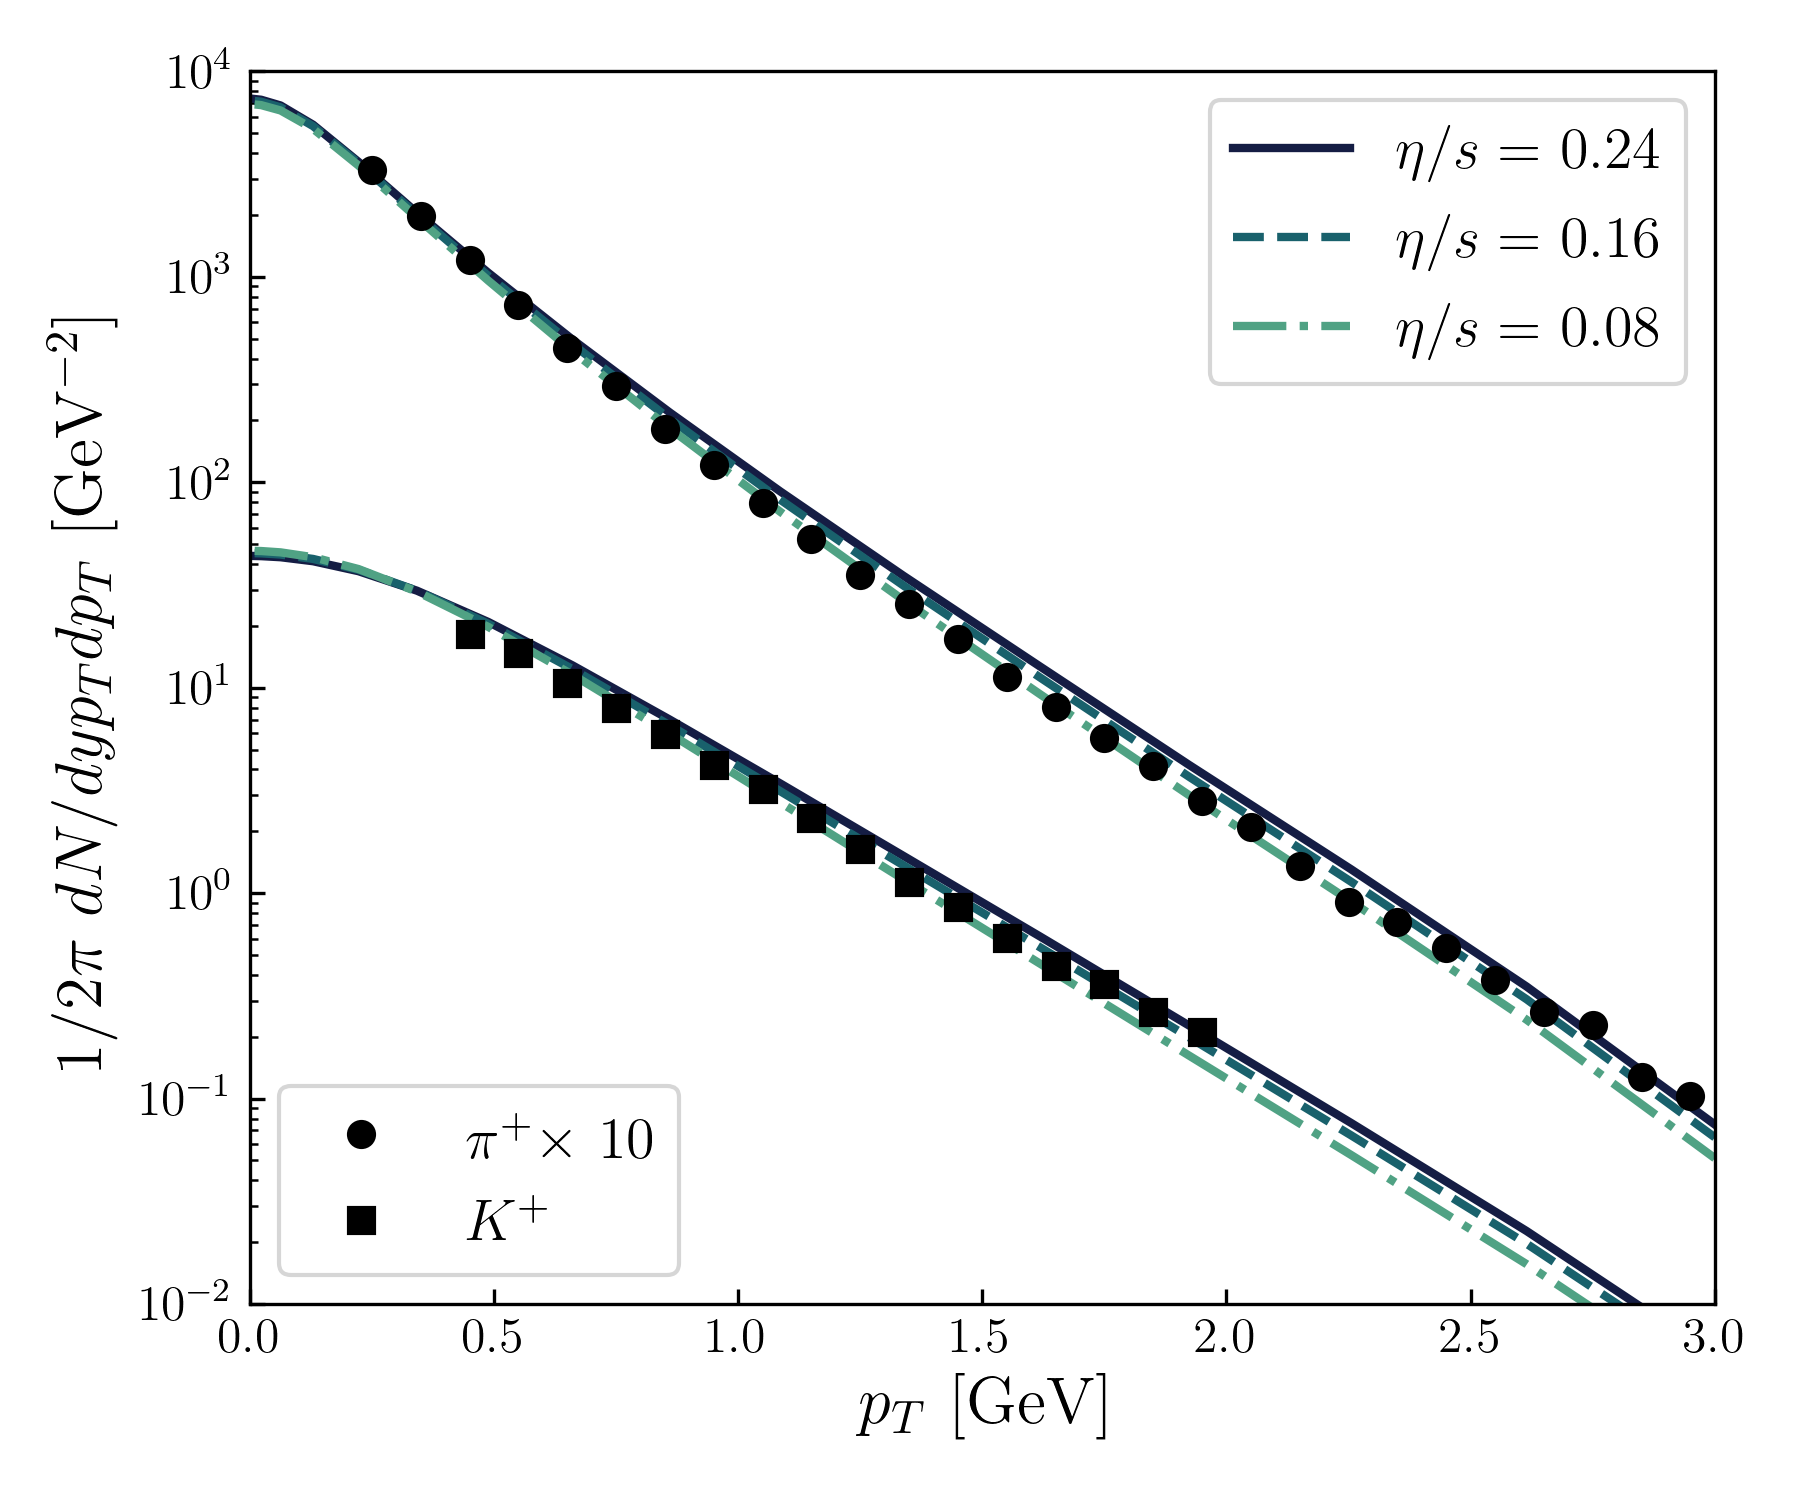
\includegraphics[width=\textwidth]{images/plot_etas_dep.png}
	\caption{\normalsize Transverse momentum spectra for positively charged pions and kaons of $0$-$5\%$ centrality, with fixed $s_\text{factor}=1.6$ and $T_\text{fo}=180$ MeV but varying $\eta/s$. The results are compared to {\sffamily PHENIX} data \cite{Adler:2003cb}. The shear viscosity correction $\delta f_\text{shear}$ is included. Increasing $\eta/s$ leads to flatter spectra.} 
\end{figure}

\begin{figure}[!hbt]
	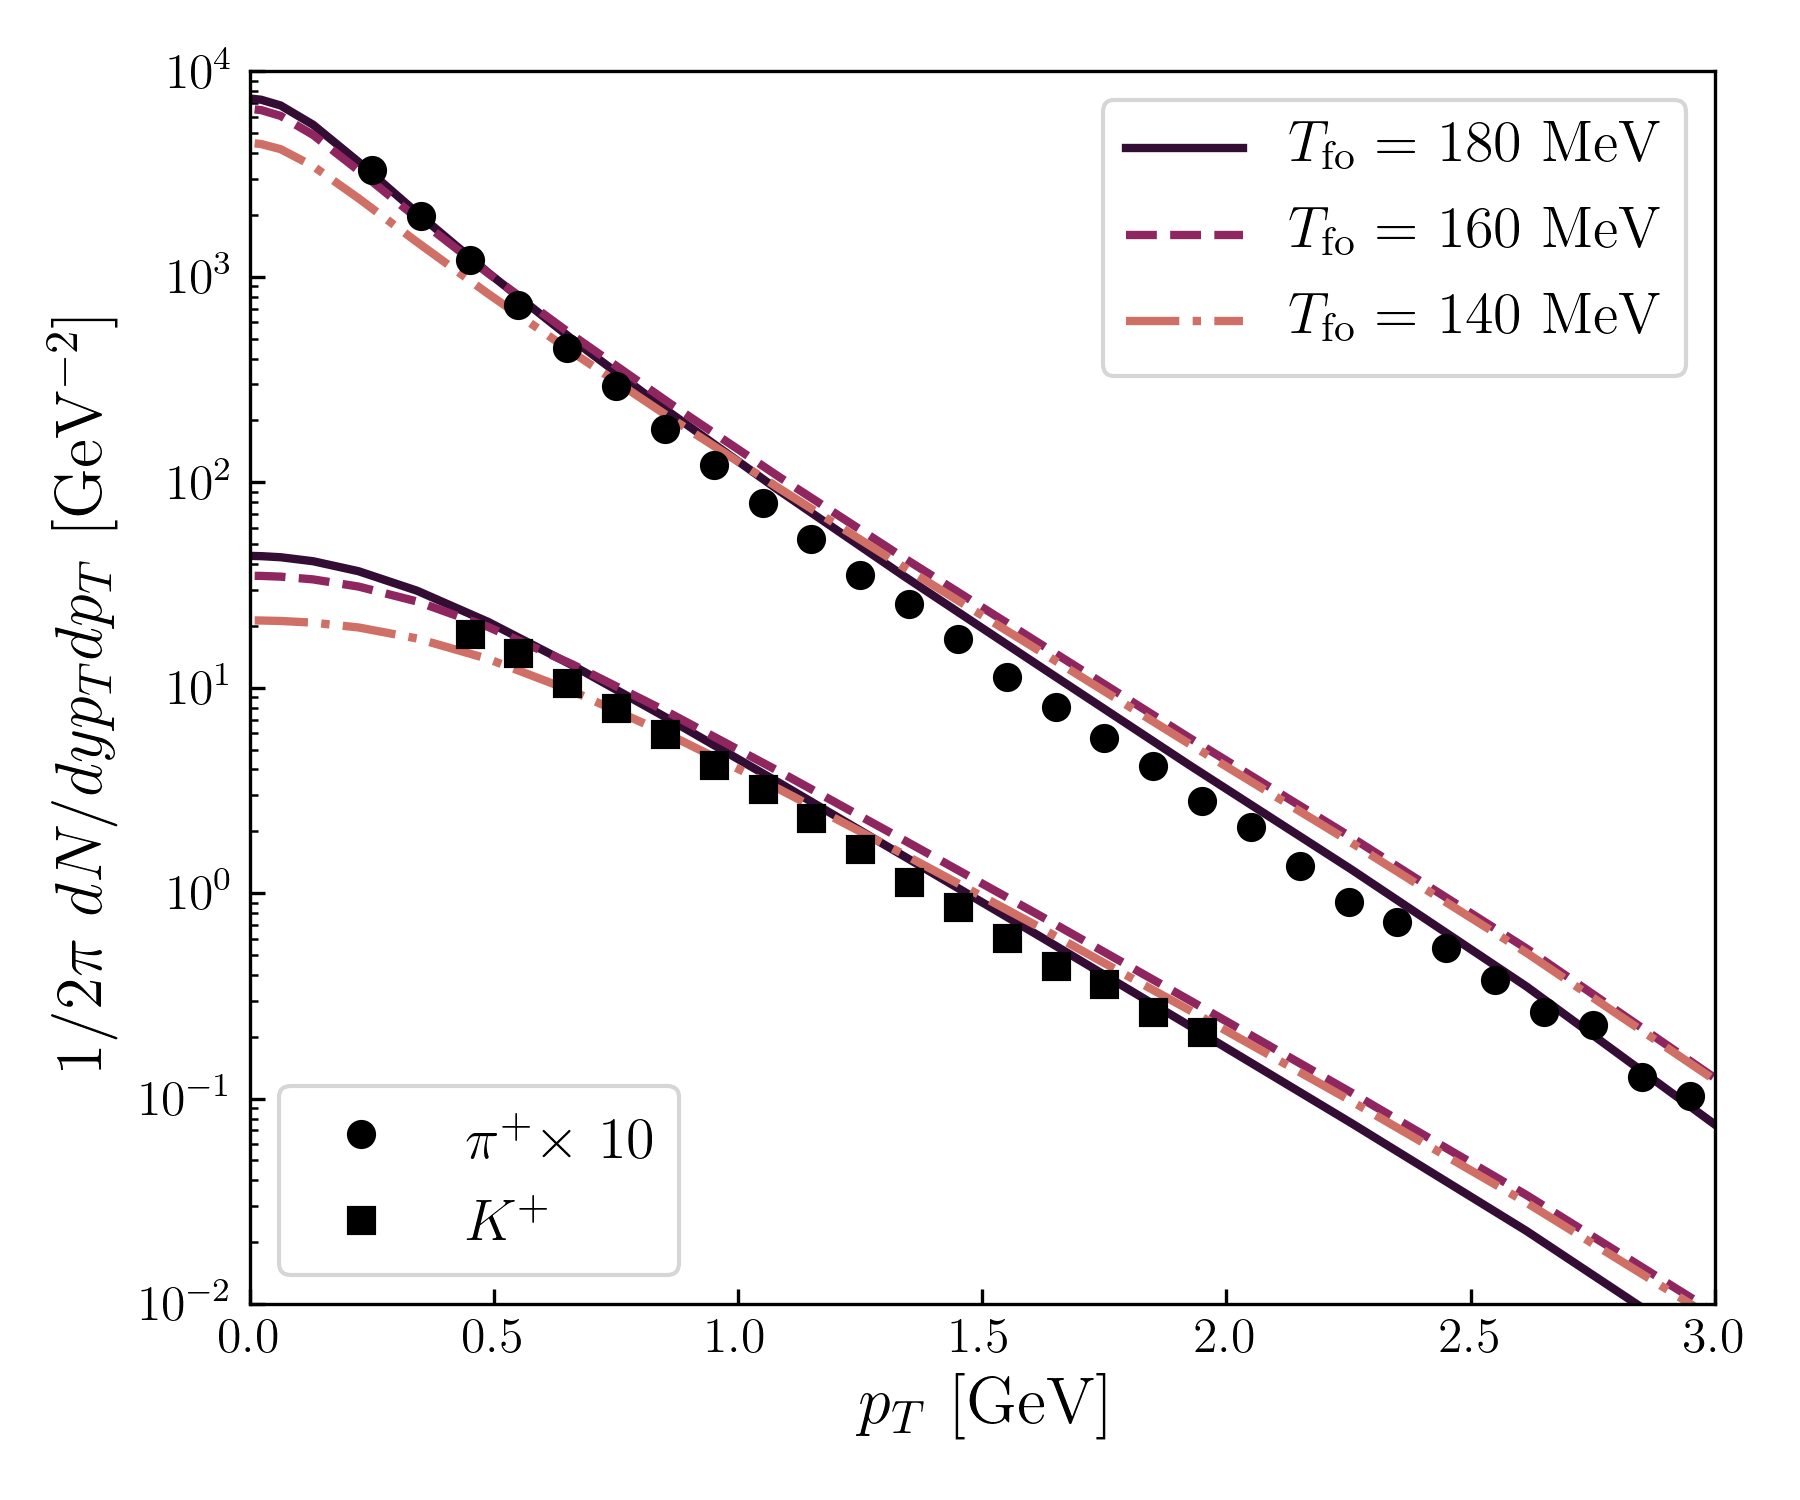
\includegraphics[width=\textwidth]{images/plot_tfo_dep.png}
	\caption{\normalsize Transverse momentum spectra for positively charged pions and kaons of $0$-$5\%$ centrality, with fixed $s_\text{factor}=1.6$ and $\eta/s=0.24$ MeV but varying $T_\text{fo}$. The results are compared to {\sffamily PHENIX} data \cite{Adler:2003cb}. The shear viscosity correction $\delta f_\text{shear}$ is included. Increasing $T_\text{fo}$ leads to steeper spectra.} 
\end{figure}

\begin{figure}[!hbt]
	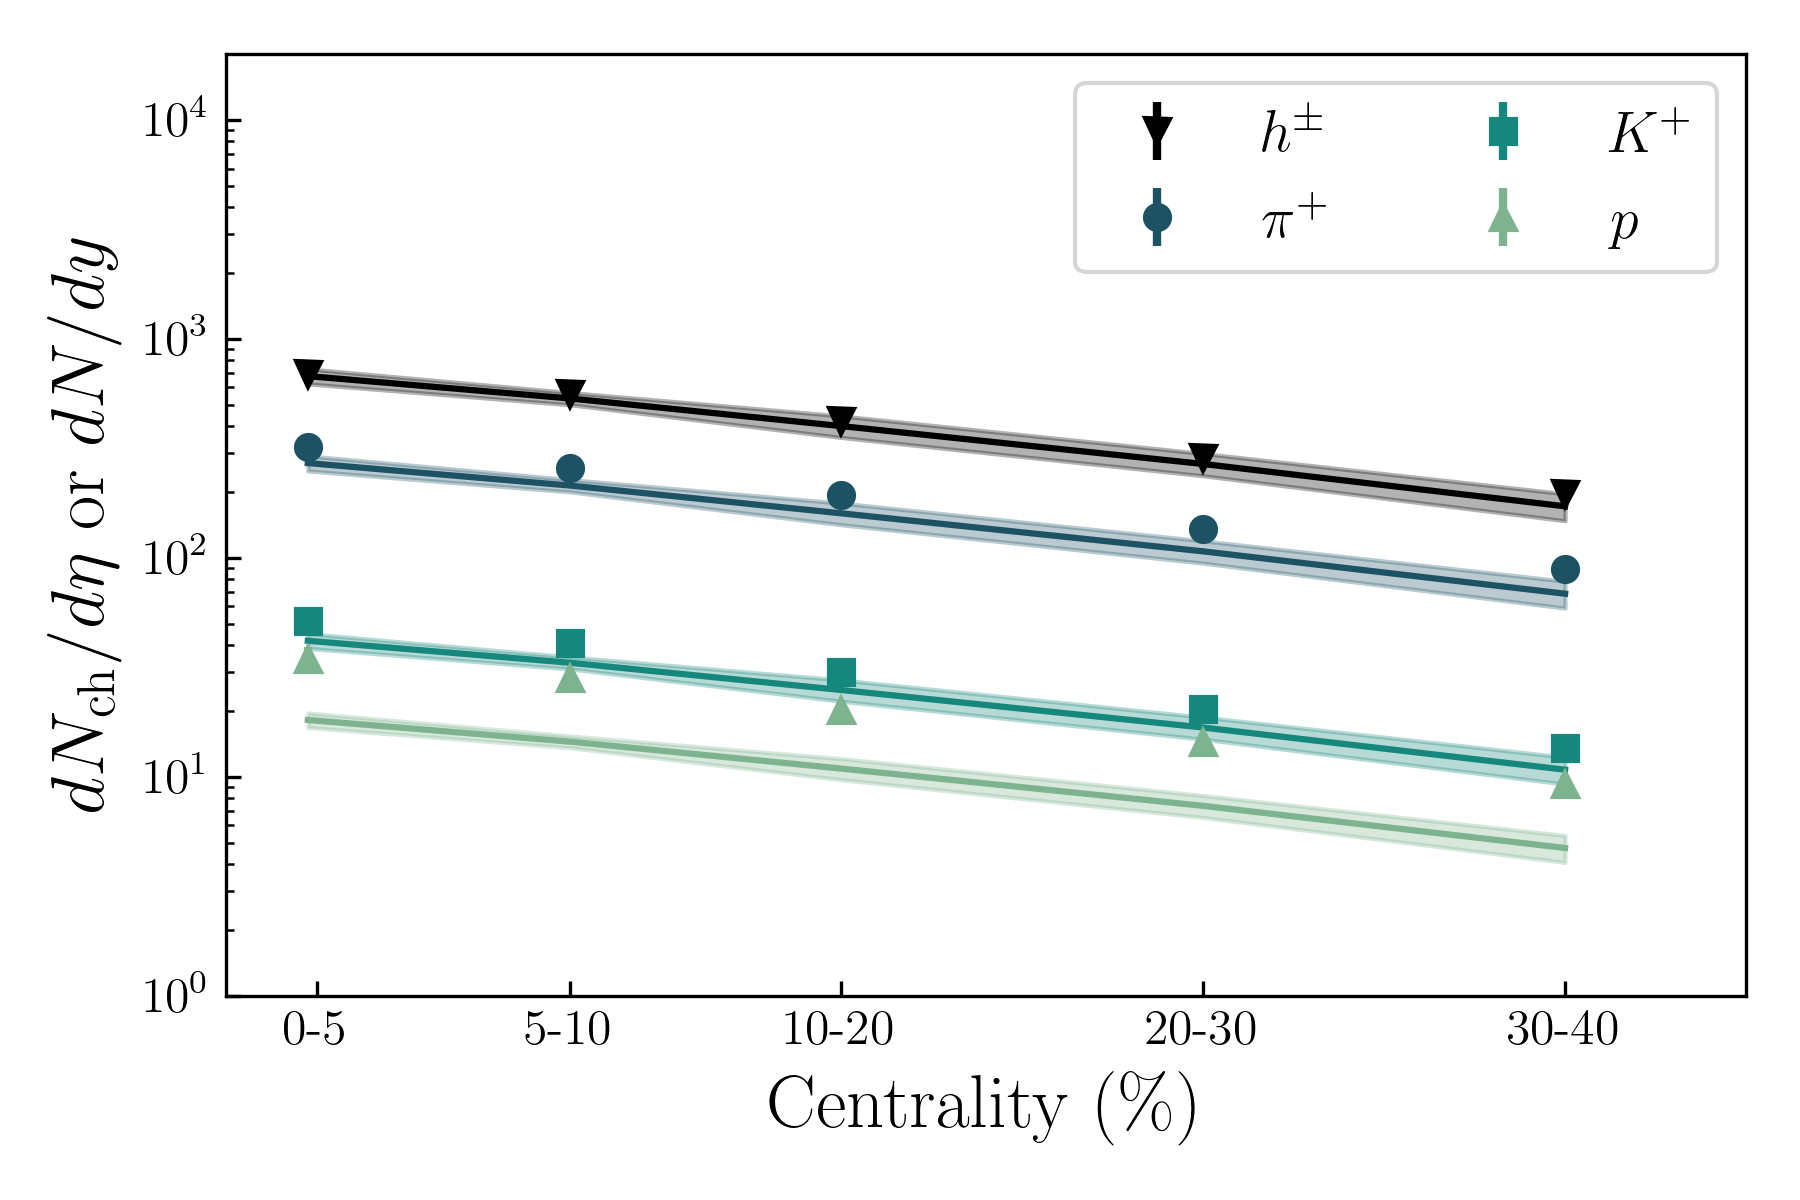
\includegraphics[width=\textwidth]{images/dn_cent_shear.png}
	\caption{\normalsize Charged particle multiplicity for all hadrons and positively charged pions, kaons and protons at different centralities. Data is taken from the tables provided in \cite{Abelev:2008ab}. The proton multiplicity is not well reproduced. In \cite{ryubulk} coupling {\sffamily MUSIC} to {\sffamily UrQMD} fixes this issue.} 
\end{figure}

\begin{figure}[!hbt]
	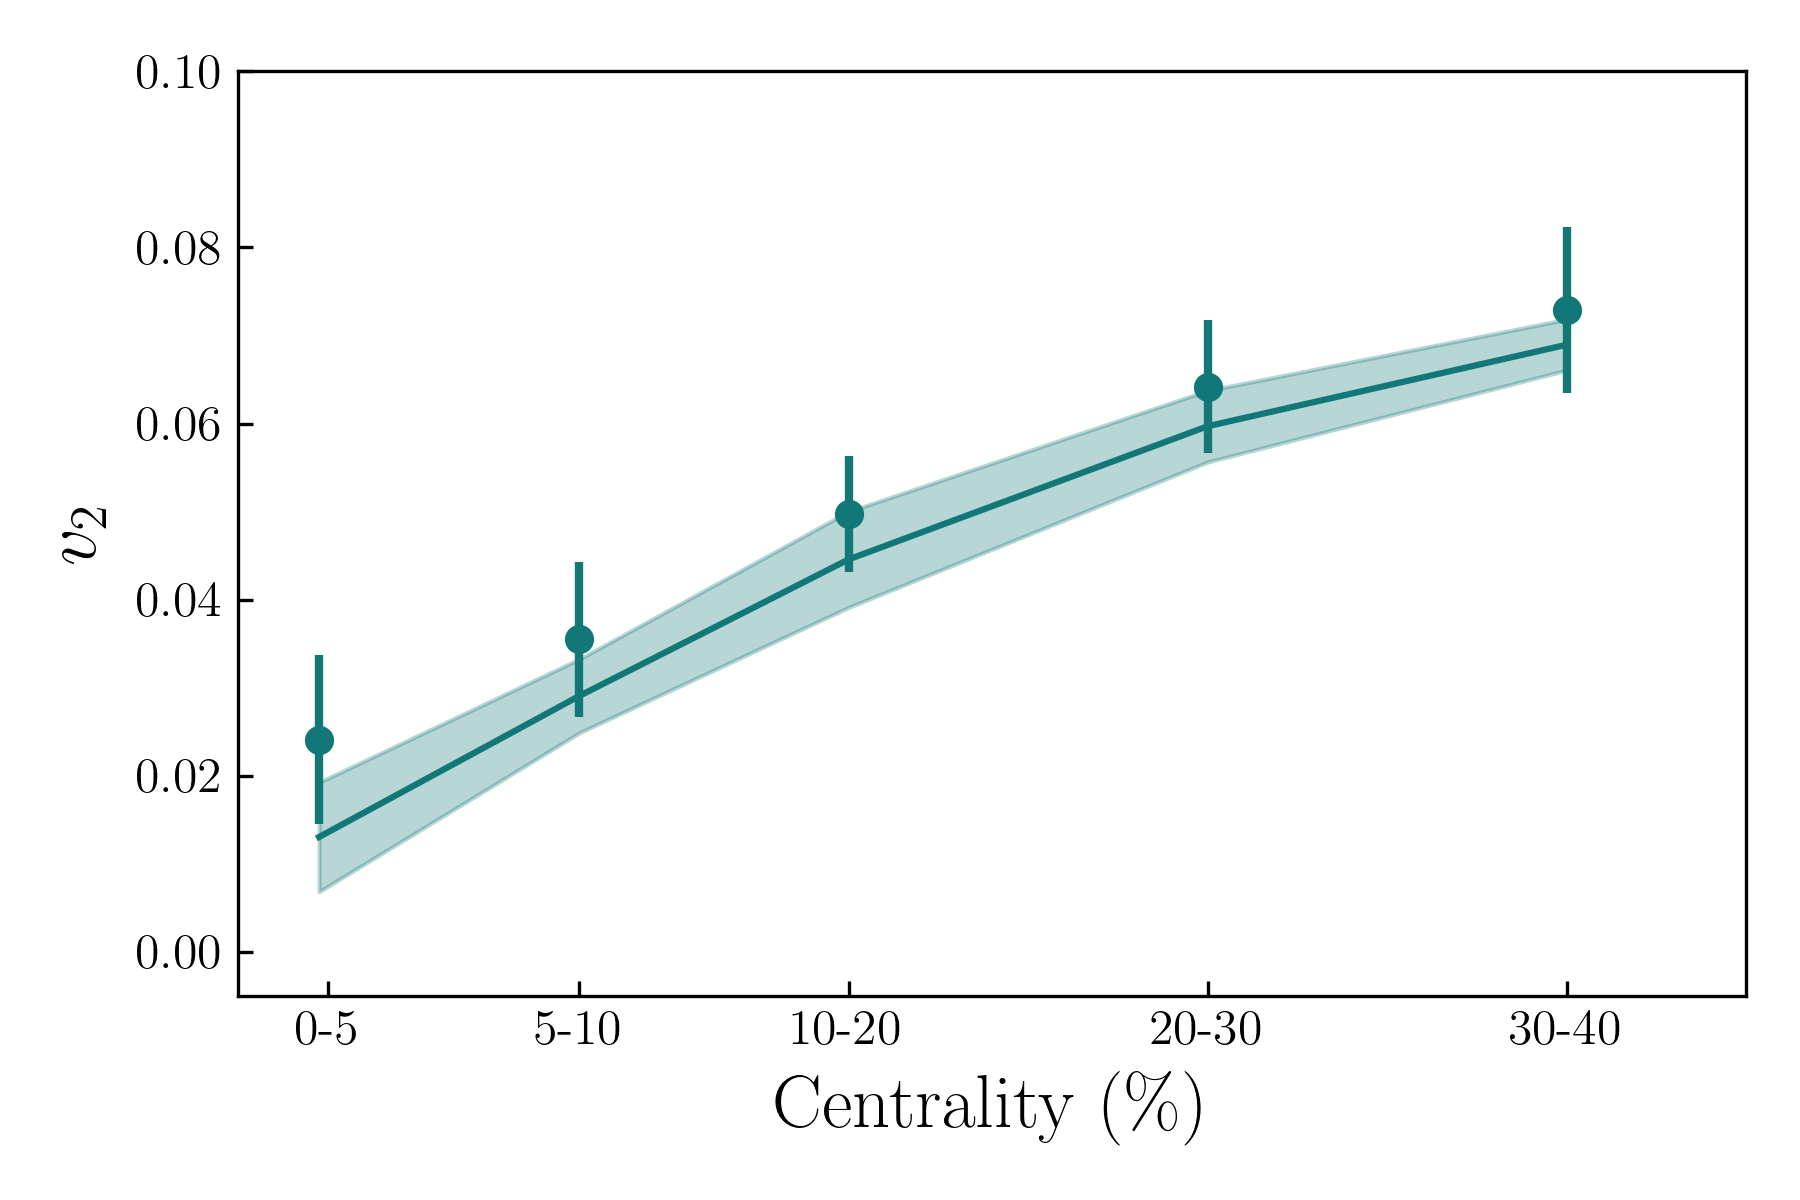
\includegraphics[width=\textwidth]{images/vn_cent.png}
	\caption{\normalsize Transverse momentum integrated elliptic flow of charged hadrons as a function of centrality. Data is taken from \cite{Abelev:2008ae}.} 
\end{figure}

\begin{figure*}[h!]
	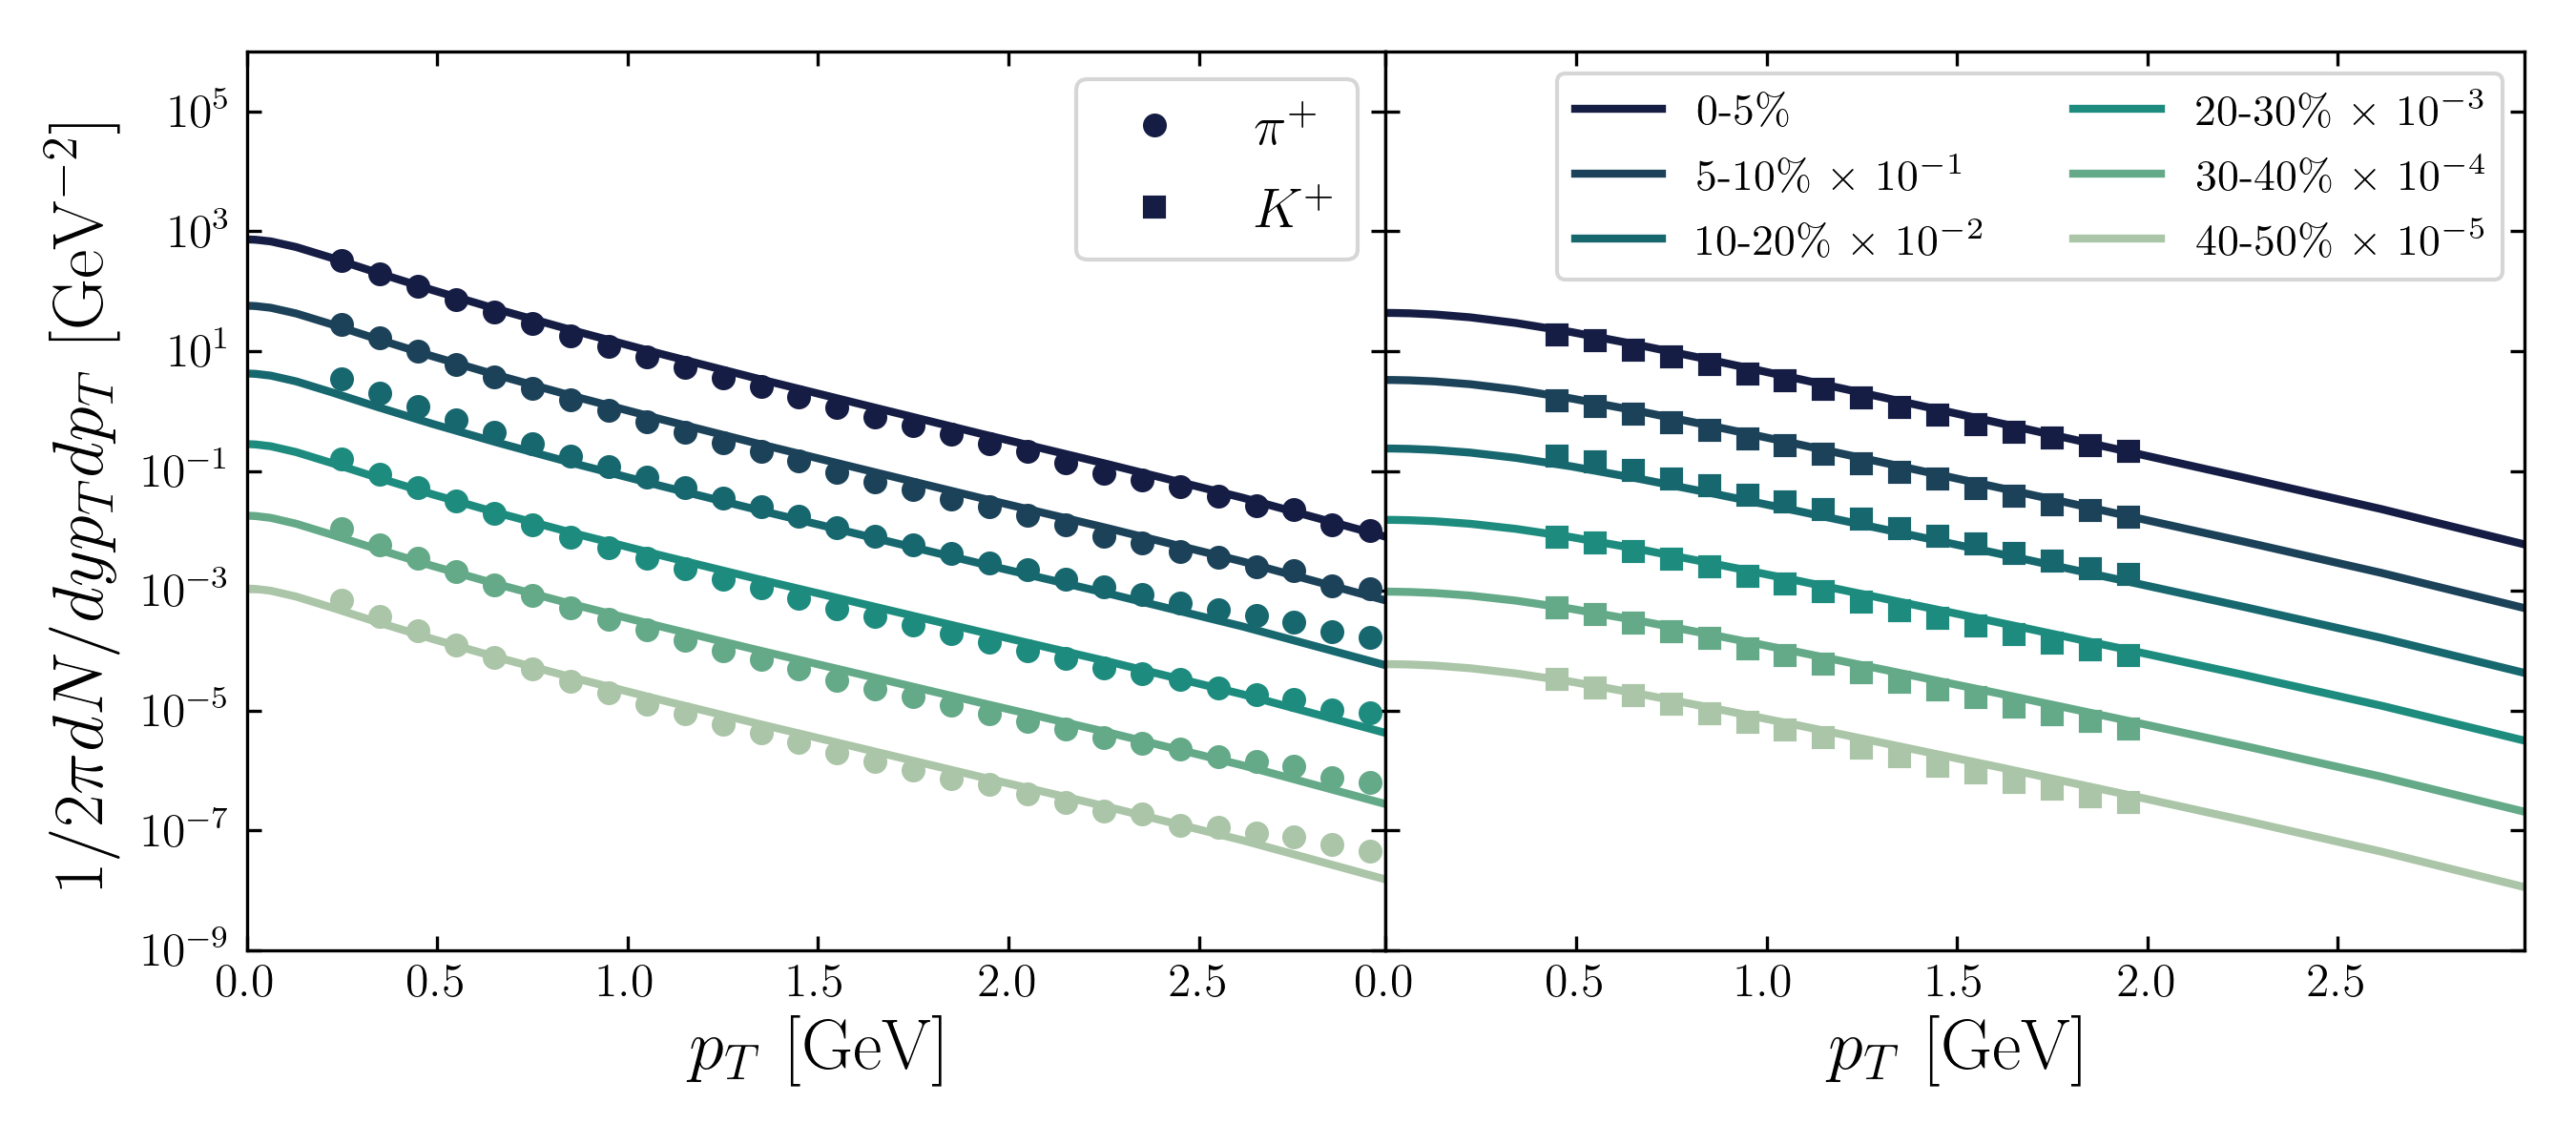
\includegraphics{images/plot_ptspectra_shear.png}
	\caption{\normalsize Transverse momentum spectra for positively charged pions and hadrons at different centralities. The results are compared to {\sffamily PHENIX} data \cite{Adler:2003cb}.}
\end{figure*}

\begin{figure}[!hbt]
	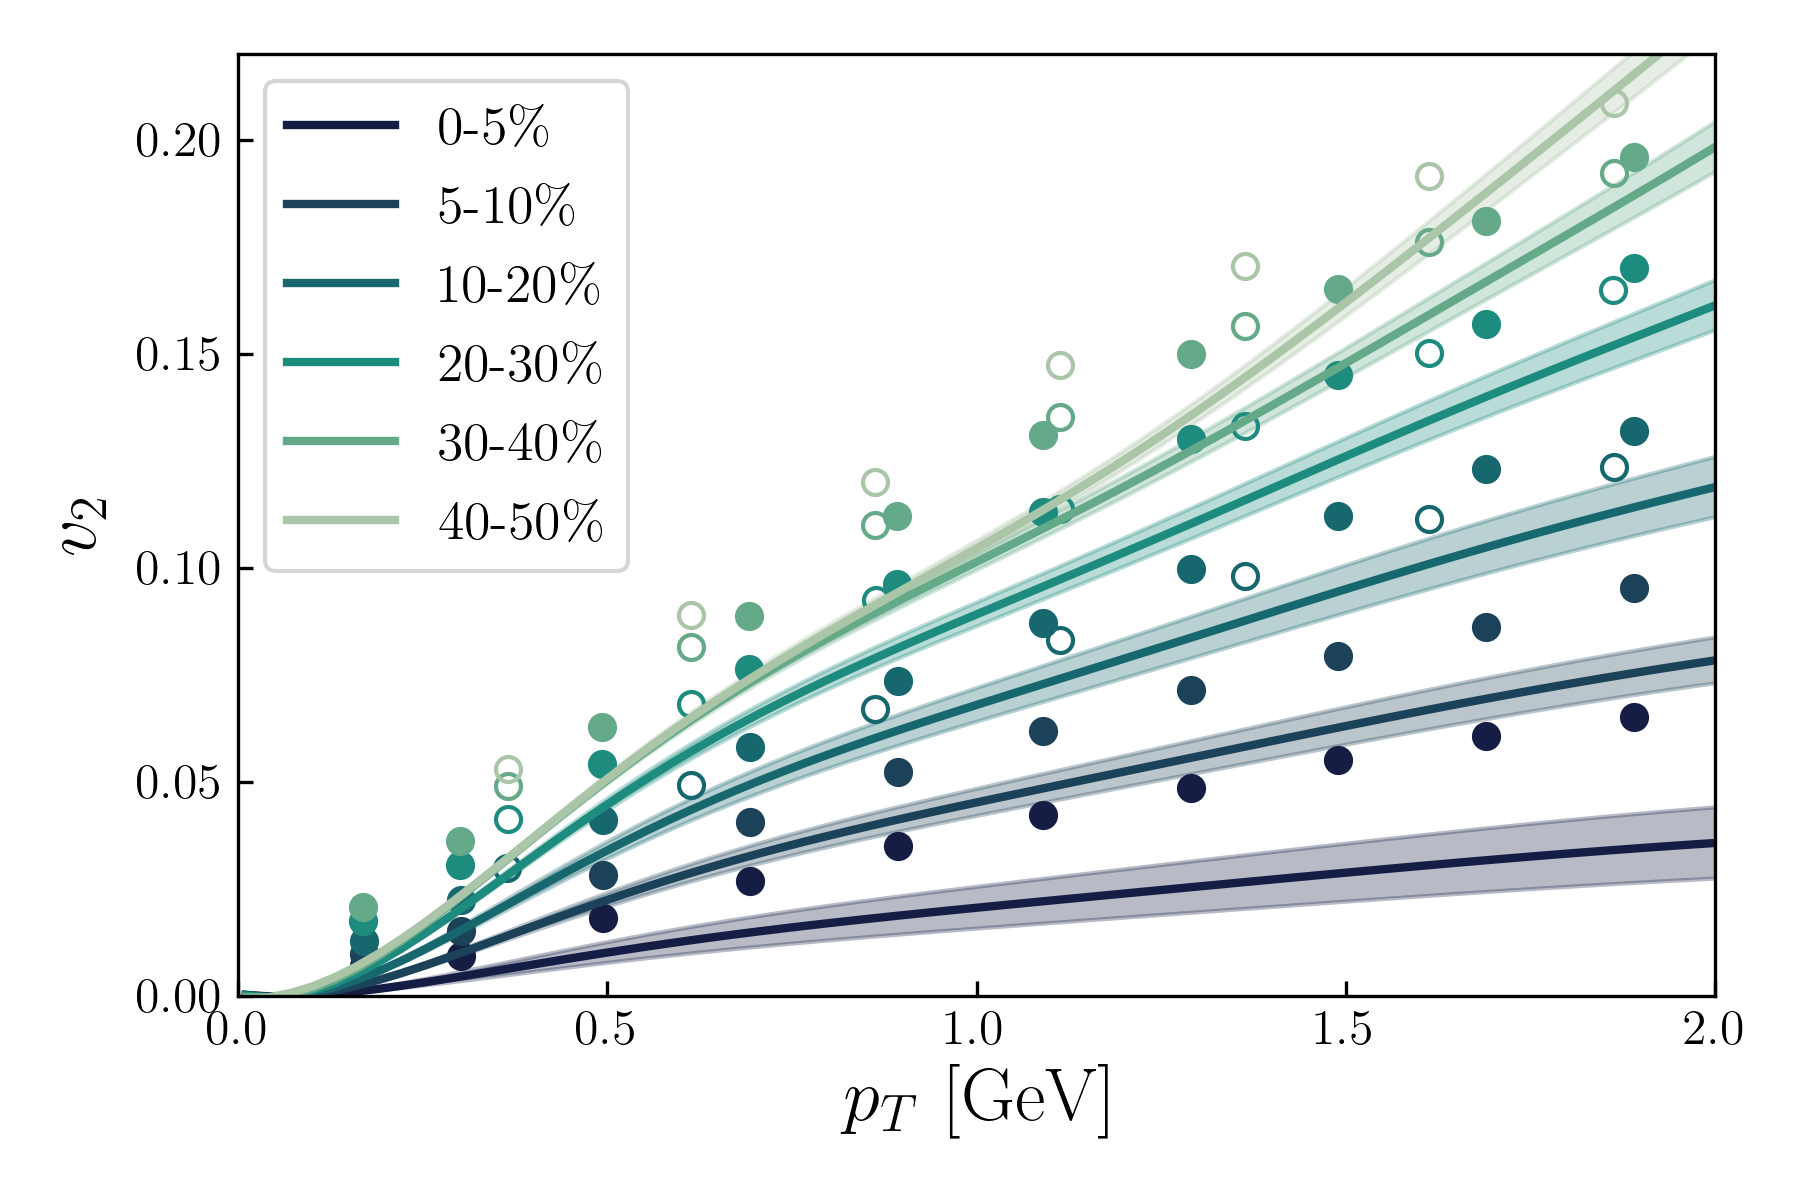
\includegraphics[width=\textwidth]{images/vn_pt.png}
	\caption{\normalsize Differential elliptic flow for charged hadrons at different centralities. The open symbols represent {\sffamily PHENIX} data points \cite{Adare:2011tg} whereas the filled correspond to {\sffamily STAR} data \cite{Adams:2004bi}.} 
\end{figure}

\newpage
\subsubsection*{Shear and bulk viscosities}
The minimal bayesian study described previously lead to the best fit parameters $s_\text{factor}=1.6$, $\eta/s=0.1$ and $T_\text{fo}=180$ MeV when bulk viscosity is also considered.

\begin{figure}[!hbt]
    \figcolor{tealblue}
	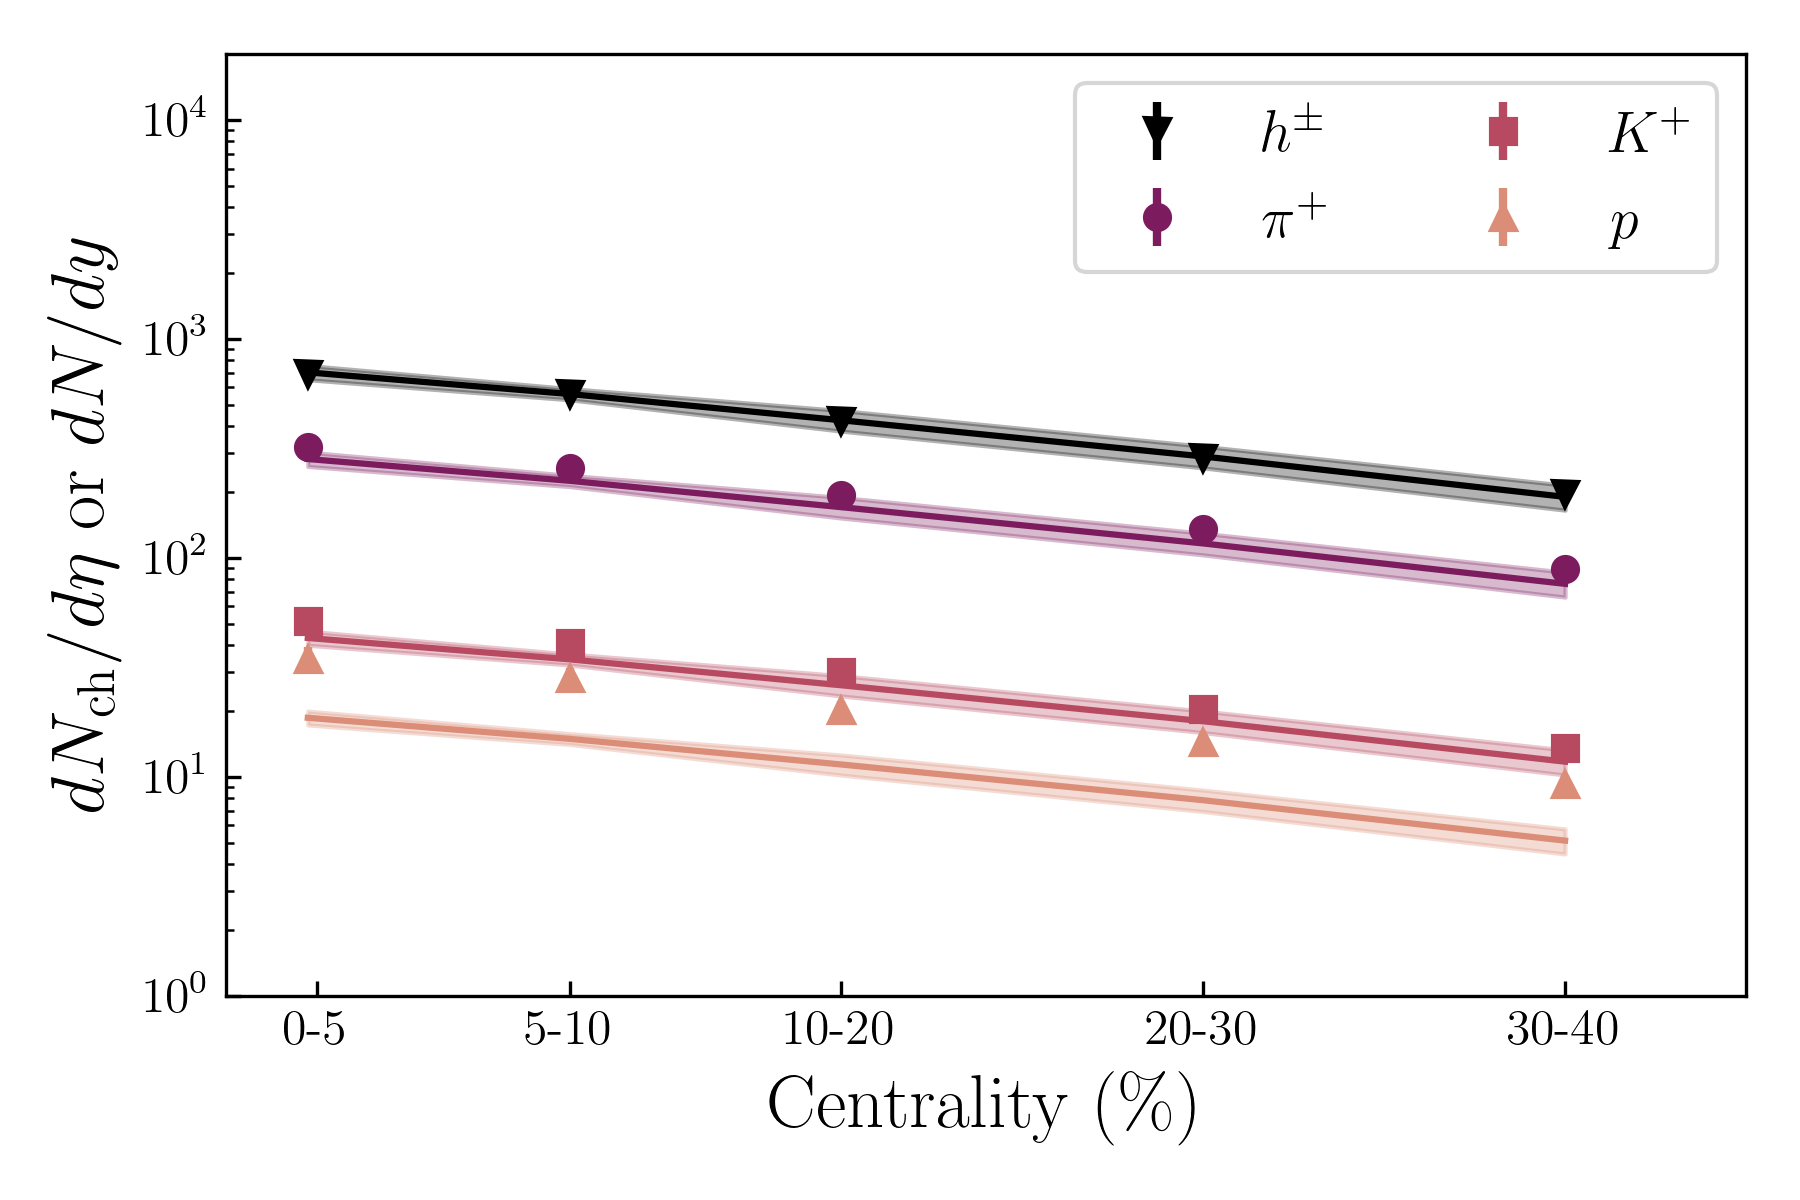
\includegraphics[width=\textwidth]{images/dn_cent_bulk.png}
	\caption{\normalsize Charged particle multiplicity for all hadrons and positively charged pions, kaons and protons at different centralities. Data is taken from the tables provided in \cite{Abelev:2008ab}. } 
\end{figure}

\begin{figure}[!hbt]
    \figcolor{tealblue}
	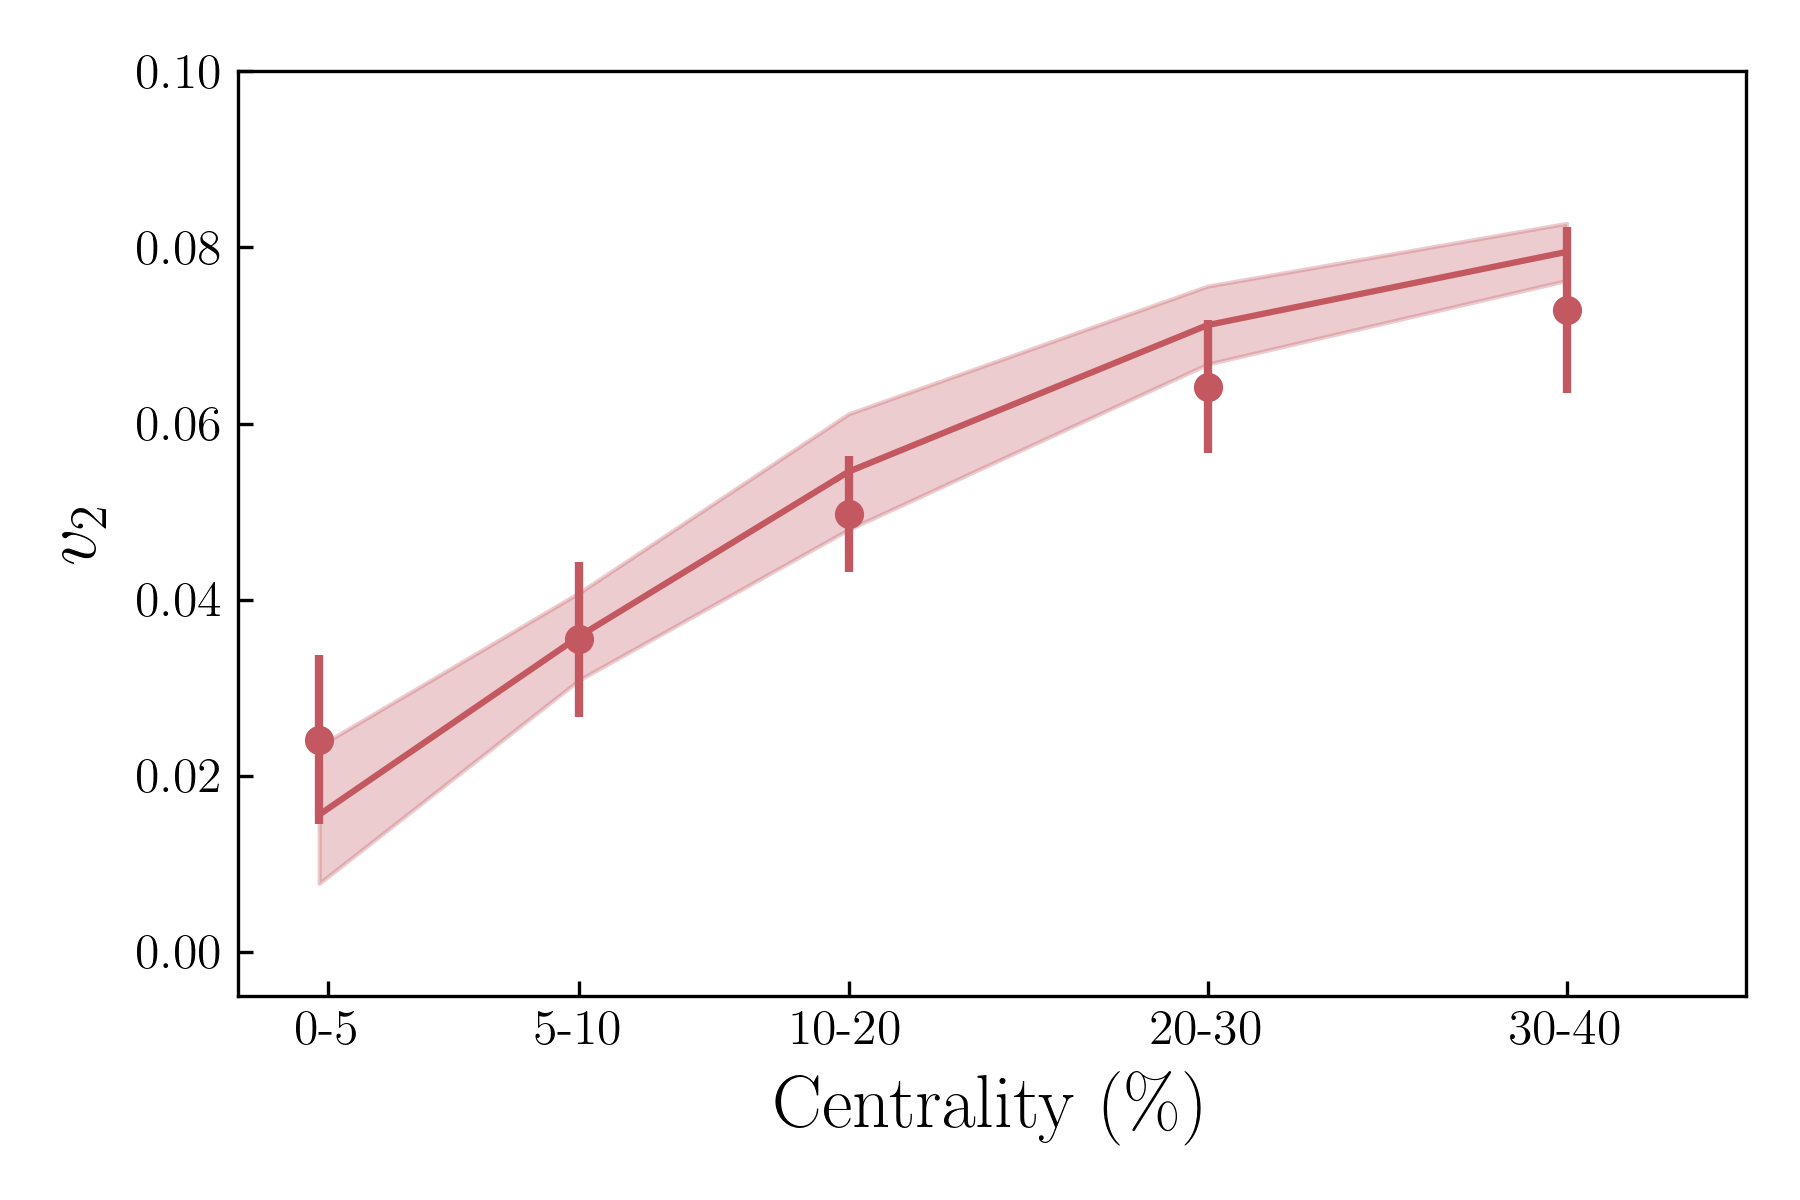
\includegraphics[width=\textwidth]{images/vn_cent_bulk.png}
	\caption{\normalsize Transverse momentum integrated elliptic flow of charged hadrons as a function of centrality. Data is taken from \cite{Abelev:2008ae}.} 
\end{figure}

\begin{figure*}[h!]
    \figcolor{tealblue}
	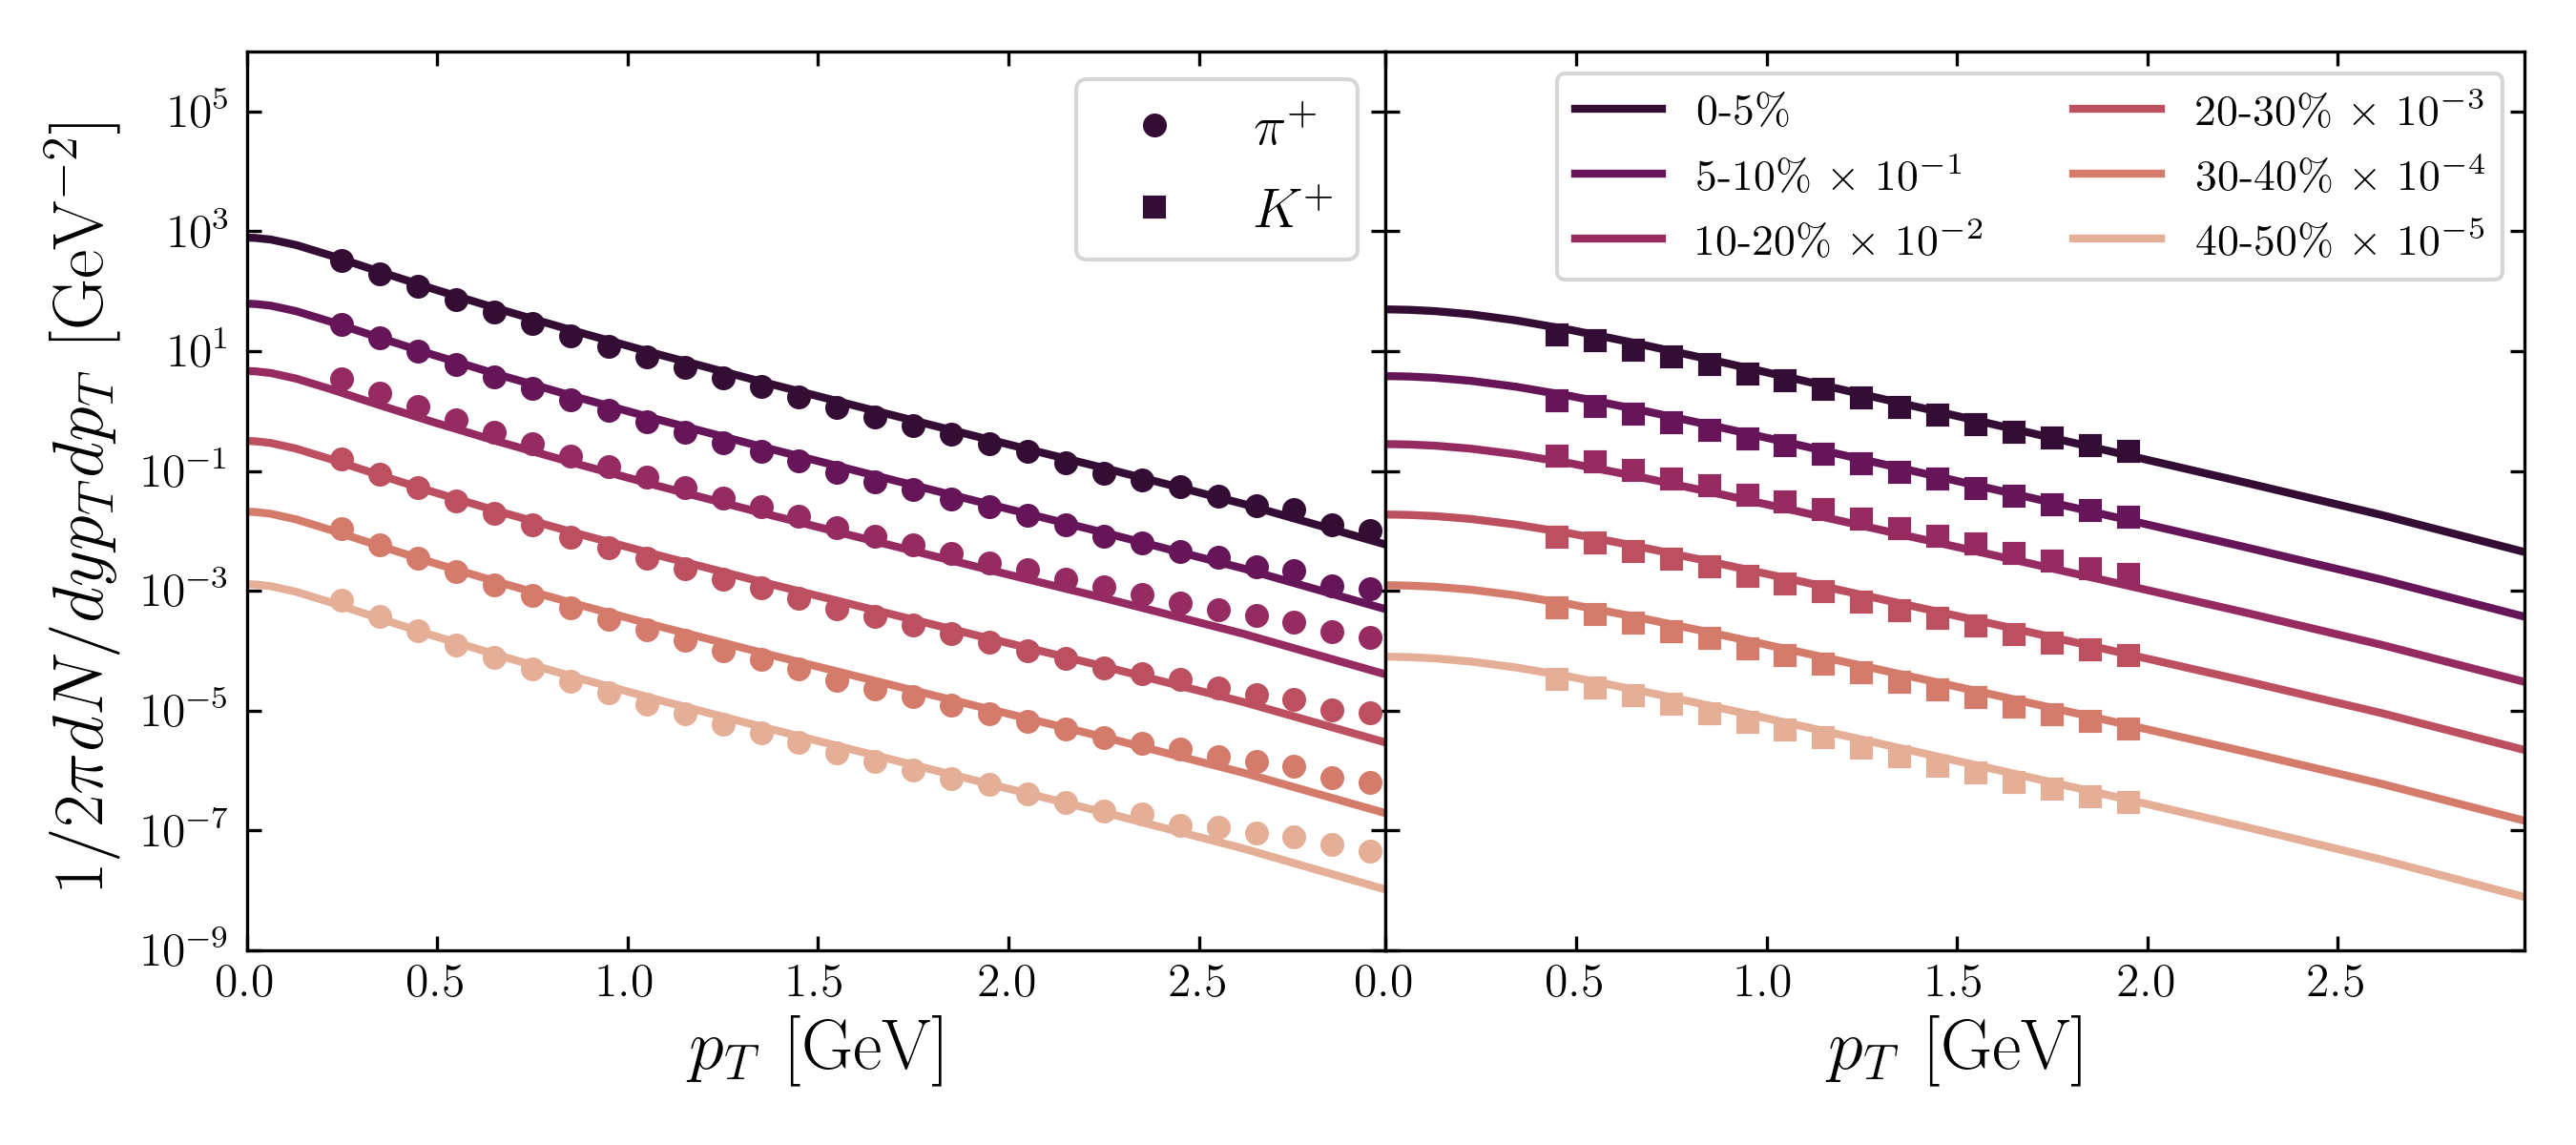
\includegraphics{images/plot_ptspectra_bulk.png}
	\caption{\normalsize Transverse momentum spectra for positively charged pions and hadrons at different centralities. The results are compared to {\sffamily PHENIX} data \cite{Adler:2003cb}.}
\end{figure*}

\begin{figure}[!hbt]
    \figcolor{tealblue}
	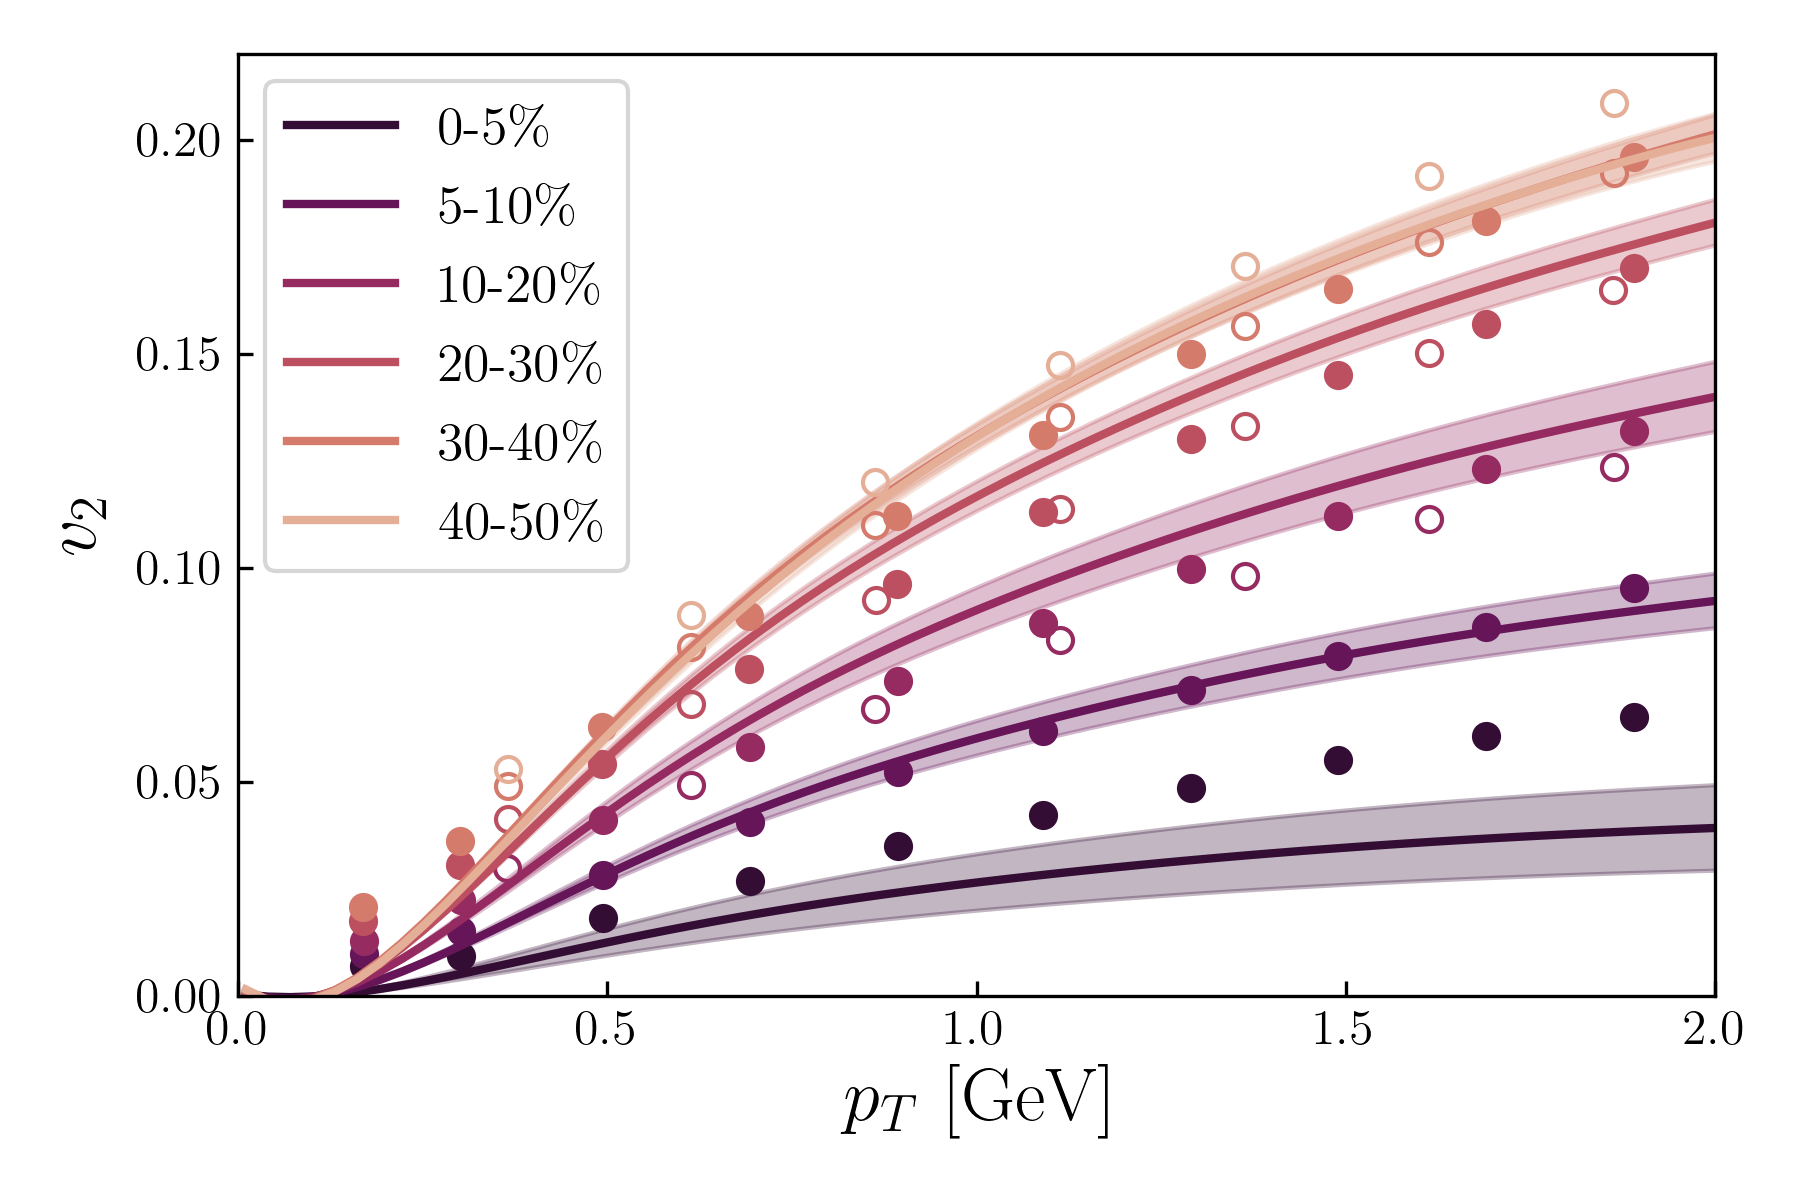
\includegraphics[width=\textwidth]{images/vn_pt_bulk.png}
	\caption{\normalsize Differential elliptic flow for charged hadrons at different centralities. The open symbols represent {\sffamily PHENIX} data points \cite{Adare:2011tg} whereas the filled correspond to {\sffamily STAR} data \cite{Adams:2004bi}.} 
\end{figure}


% \begin{summary}[]
% [...]
% \end{summary}
